\begin{frame}
	\frametitle{Exkurs: Eigenschaften des Wassers - Phasendiagramm}

	\begin{figure}
		\centering
		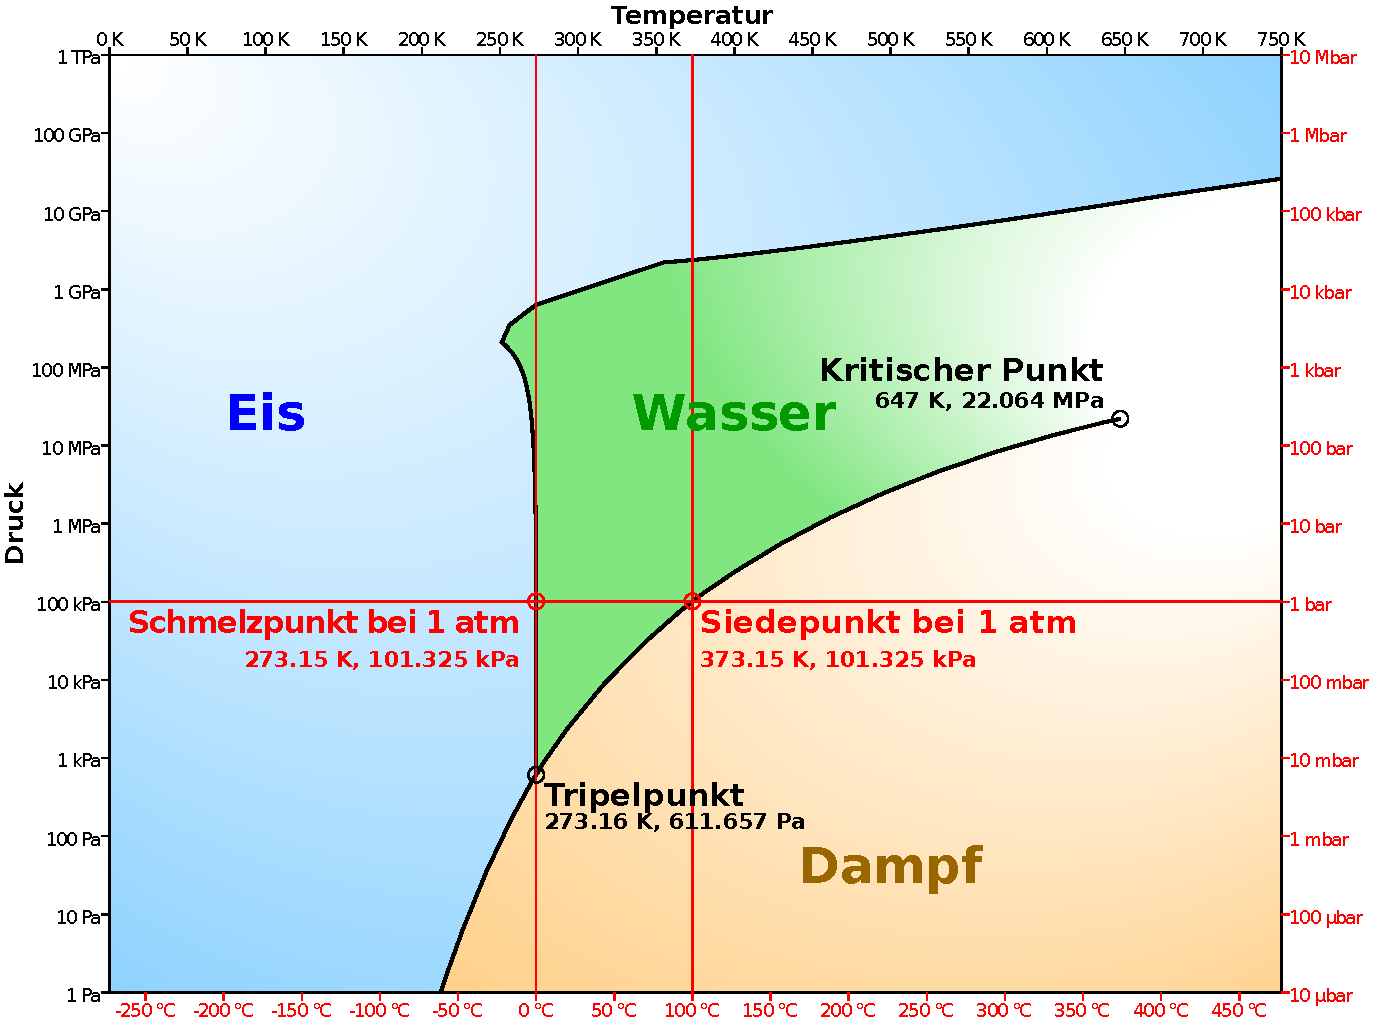
\includegraphics[width=0.7\linewidth]{bilder/Phase_diagram_of_water_simplified.pdf}
		\caption{Phasendiagramm von Wasser, Quelle: Cmglee nach LSBU}
	\end{figure}

	\note{
		\begin{itemize}
			\item[] Wasser kann in drei Phasen/Aggregatszuständen vorliegen: Gasförmig (Dampf), flüssig und fest (Eis)
			\item[] Besonderheit: Kommen alle drei in nennenswerter Menge in unserer Umwelt vor
			\item[] Phase hängt von Temperatur und Druck ab $\rightarrow$ Achsen des Phasendiagramms (Druck als log-Skala)
			\item[] Übergang von einer Pahsen zur anderen abrubt
			\item[] Punkte von besonderer Bedeutung:
			\begin{itemize}
				\item[] Schmelz- und Siedepunkt bei 1\, atm (Normaldruck) definierendie Celsius Temperaturskala
				\item[] Trippelpunkt: Punkt an dem Wasser in allen drei Phasen vorliegen kann (im thermodynamischen Gleichgewicht)
				\item[] Kritischer Punkt: Ab diesem Punkt gehen gasförmige und flüssige Phase in einander über
			\end{itemize}
		\item[] Dichteanomalie Besonderheit von Wasser
		\item[$\rightarrow$] Bei konstanter Temperatur kann die Phase von flüssig zu fest und wieder zu flüssig wechseln
		\item[$\rightarrow$] Wasser hat bei $\approx\SI{4}{\degreeCelsius}$ größe Dichte, darüber und darunter sinkt sie. Bei vielen anderen Stoffe steigt Dichte mit sinkender Temperatur
		\end{itemize}
	}
\end{frame}

\begin{frame}
	\frametitle{Interaktion Kryosphäre und Lithosphäre}

	\begin{figure}
		\centering
		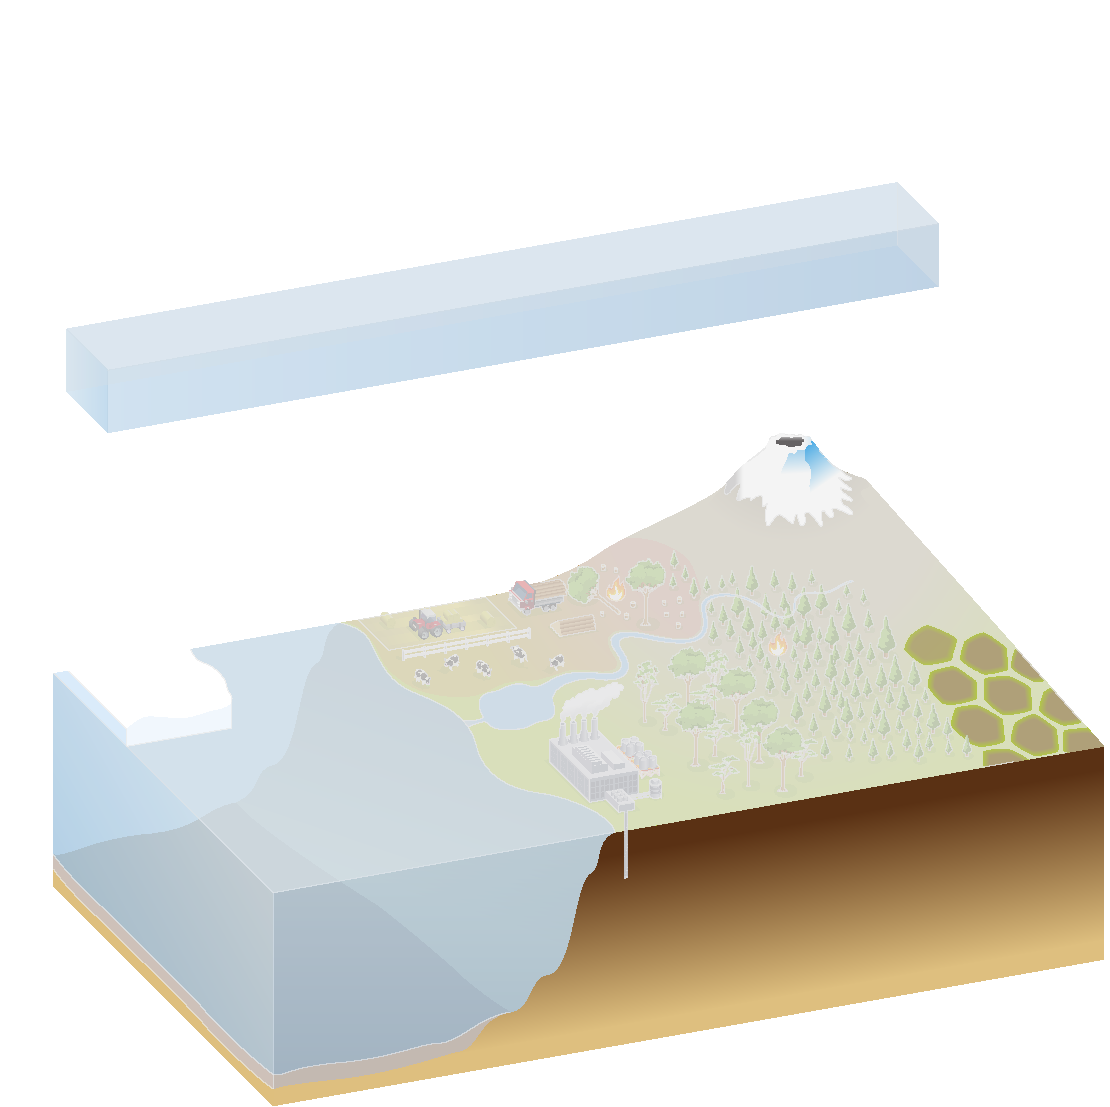
\includegraphics[trim={1cm 0cm 0cm 3cm}, clip, width=0.55\linewidth]{%
				bilder/climate_components/global_climate_components_interaction_kryo_litho.pdf}
		\caption{Interaktion zwischen Kryosphäre und Lithosphäre}
	\end{figure}

	\note{
	\begin{itemize}
		\item[] An der Unterseite des Eisschildes, am Kontakt zwischen Fels und Eis, gibt es einen geothermischen Wärmeeintrag
		\item[$\rightarrow$] Temperatur entlang der Eissäule nimmt mit der Tiefe zu.
		\item[$\rightarrow$] Druckschmelzpunkt kann erreicht werden, sodass flüssiges Wasser an der Grenzschicht vorliegt.
		\item[$\rightarrow$] Schmierfilm, für den Eisschild, der zur schnellen Destabilisierung des westantarktischen Eisschildes führen kann.
		\item[] Weiterhin: Absenkung des Fels durch Gewicht des Eises um etwa \SI{30}{\percent} der Eisdicke
		\item[$\rightarrow$] Nordamerika und Skandinavien heben sich immer noch infolge der Entlastung der eiszeitlichen Eisschilde
	\end{itemize}
	}
\end{frame}
